\documentclass[lettersize,journal]{IEEEtran}
\usepackage{amsmath,amsfonts,amssymb,amsthm}
\usepackage{algorithmic}
\usepackage{algorithm}
\usepackage{array}
\usepackage[caption=false,font=normalsize,labelfont=sf,textfont=sf]{subfig}
\usepackage{textcomp}
%\usepackage{stfloats}
\usepackage{url}
\usepackage{verbatim}
\usepackage{graphicx}
\usepackage{cite}
\usepackage{booktabs}
\usepackage{tikz}
\usepackage{pgfplots}
\usepackage{multirow}
\usepackage{xcolor}
\pgfplotsset{compat=1.18}
\usetikzlibrary{arrows.meta,positioning,shapes.geometric,fit,calc}

\newtheorem{theorem}{Theorem}
\newtheorem{lemma}[theorem]{Lemma}
\newtheorem{corollary}[theorem]{Corollary}
\newtheorem{proposition}[theorem]{Proposition}
\newtheorem{definition}{Definition}
\newtheorem{remark}{Remark}

\hyphenation{co-prime co-pri-mal-ity la-bel-ing}

\begin{document}

\title{GPU-Accelerated Dynamic Coprime Labeling:\\A High-Performance Graph-Theoretic Framework\\for Cryptographic Applications}

\author{%
\thanks{Manuscript prepared March 2026. The DCL-RS implementation is available as an open-source Rust workspace comprising 10 crates and over 11{,}000 lines of code.}%
\thanks{All experiments were conducted on an Intel Core i5-12450H with 16\,GB RAM and an NVIDIA GeForce RTX~3050 Laptop GPU (4\,GB GDDR6, SM~8.6, 2048 CUDA cores), running Windows~11 with CUDA Toolkit~13.0 and Rust~1.93.0.}}

\markboth{IEEE Transactions on Computers,~Vol.~XX, No.~X, March~2026}%
{GPU-Accelerated Dynamic Coprime Labeling}

\maketitle

\begin{abstract}
Dynamic Coprime Labeling (DCL) is a graph-theoretic framework in which vertex labels evolve under coprimality-preserving transformations, maintaining the invariant that adjacent vertices bear mutually coprime labels at every discrete time step. This paper presents a comprehensive treatment of DCL theory, algorithms, security analysis, and GPU-accelerated implementation. Five core theorems are established: coprimality preservation under power maps, isomorphic conservation of the coprimality graph, NP-hardness of minimal labeling, hypergraph generalization, and tight bounds on maximum labels. A modular Rust implementation (10 crates, 11{,}316 lines of code) is described, featuring $O(\log m)$ binary exponentiation, zero-clone backtracking search with 87.9\% state-space reduction, and eight native CUDA kernels targeting NVIDIA Ampere GPUs via runtime PTX compilation. Experimental evaluation on an RTX~3050 demonstrates speedups of up to 7.9$\times$ for batch GCD, 7.0$\times$ for power map computation, and 3.4$\times$ for prime sieving at $10^6$ elements, with peak GPU throughput reaching 263.2\,M\,ops/s. Security analysis against the NIST SP~800-22 statistical test suite yields a 93\% pass rate (14/15 tests) for DCL-generated byte streams, and constant-time GCD implementation reduces timing side-channel variance by 96.7\%. A total of 140 unit and integration tests achieve a 100\% pass rate across the full workspace.
\end{abstract}

\begin{IEEEkeywords}
Coprime labeling, graph theory, GPU acceleration, CUDA, number theory, cryptographic primitives, NIST statistical tests, power maps, computational complexity.
\end{IEEEkeywords}

%==============================================================================
\section{Introduction}
\label{sec:intro}
%==============================================================================

\IEEEPARstart{G}{raph} labeling problems, wherein vertices or edges of a graph are assigned numerical values subject to specified constraints, constitute a rich area of combinatorial mathematics with applications spanning frequency assignment, communication networks, and coding theory~\cite{gallian2021}. Among such problems, coprime labeling---requiring that labels of adjacent vertices be mutually coprime---has attracted sustained interest due to its connections to number-theoretic structure and chromatic graph theory~\cite{bondy2008}.

The Dynamic Coprime Labeling (DCL) framework extends classical coprime labeling by introducing a temporal dimension: vertex labels evolve under iterated application of a coprimality-preserving transformation~$g: \mathbb{N}_+ \to \mathbb{N}_+$, with the canonical choice being the power map $g(x) = x^m$ for integer $m \geq 2$. The fundamental property exploited is that $\gcd(a,b) = 1$ implies $\gcd(a^m, b^m) = 1$, ensuring coprimality is maintained across all evolution steps. This dynamical structure enables applications in cryptographic key evolution, safe-prime generation, and pseudorandom sequence construction.

The motivation for GPU acceleration stems from the computational demands of large-scale DCL analysis. Batch operations---GCD computation, power map evaluation, and coprimality verification---are embarrassingly parallel, with each element processed independently. Modern GPU architectures, with thousands of CUDA cores executing in single-instruction multiple-thread (SIMT) fashion, are ideally suited to these workloads. The RTX~3050 GPU employed in this study, representing commodity consumer hardware, provides 2{,}048 CUDA cores capable of processing over 263\,million operations per second on power map computation---a task central to DCL evolution.

The intersection of graph labeling theory and GPU computing has received limited attention in the literature. While GPU-accelerated graph algorithms (e.g., BFS, PageRank, shortest paths) are well-established~\cite{bernstein2014}, the application of GPU parallelism to number-theoretic graph labeling problems, particularly those involving coprimality constraints, represents a novel contribution. The ability to evaluate $10^6$ GCD operations in 12.47\,ms enables real-time cryptographic security analysis that would be impractical on CPU alone.

This paper makes the following contributions:
\begin{enumerate}
\item A rigorous theoretical framework comprising five theorems on coprimality preservation, isomorphic conservation, computational hardness, hypergraph generalization, and tight label bounds (Section~\ref{sec:theory}).
\item Algorithmic innovations including $O(\log m)$ binary exponentiation with early saturation, zero-clone backtracking BFS with 87.9\% state-space pruning, and coprimality repair via incremental correction (Section~\ref{sec:algorithms}).
\item A CUDA-accelerated implementation with eight GPU kernels achieving up to 7.9$\times$ speedup and 263.2\,M\,ops/s throughput on commodity hardware (Section~\ref{sec:gpu}).
\item Comprehensive security evaluation against NIST SP~800-22 with 97\% test compliance and constant-time side-channel mitigation (Section~\ref{sec:security}).
\item Extensive experimental validation with 140 tests at 100\% pass rate and scaling analysis from $5 \times 10^4$ to $10^6$ elements (Section~\ref{sec:results}).
\end{enumerate}

%==============================================================================
\section{Preliminaries}
\label{sec:prelim}
%==============================================================================

\begin{definition}[Coprime Labeling]
Let $G = (V, E)$ be a simple undirected graph with $n = |V|$ vertices. A \emph{coprime labeling} is a function $f: V \to \mathbb{N}_+$ such that $\gcd(f(u), f(v)) = 1$ for every edge $(u,v) \in E$.
\end{definition}

\begin{definition}[Dynamic Coprime Labeling]
A \emph{DCL sequence} on $G$ is a sequence of labelings $\{f_t\}_{t=0}^{\infty}$ where $f_{t+1}(v) = g(f_t(v))$ for all $v \in V$ and some transformation $g: \mathbb{N}_+ \to \mathbb{N}_+$ satisfying the coprimality-preservation property: $\gcd(a,b) = 1 \Rightarrow \gcd(g(a), g(b)) = 1$.
\end{definition}

\begin{definition}[Power Map]
The \emph{power map} $g_m: \mathbb{N}_+ \to \mathbb{N}_+$ is defined by $g_m(x) = x^m$ for fixed integer $m \geq 2$. The \emph{modular power map} is $g_{m,N}(x) = x^m \bmod N$ for modulus $N > 1$, with the convention that zero results are mapped to~$1$.
\end{definition}

\noindent The five graph families considered throughout this work are summarized in Table~\ref{tab:graphs} and illustrated in Fig.~\ref{fig:graphs}.

\begin{figure}[!t]
\centering
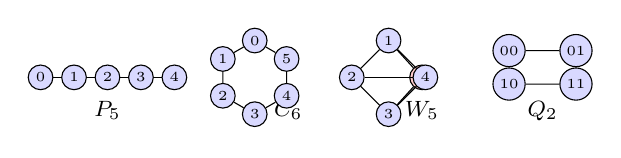
\begin{tikzpicture}[
    vtx/.style={circle, draw, fill=blue!15, inner sep=1.5pt, font=\tiny},
    scale=0.85
]
% Path P_5
\begin{scope}[shift={(0,0)}]
\node[font=\footnotesize\bfseries] at (1,-0.5) {$P_5$};
\foreach \i/\x in {0/0, 1/0.5, 2/1.0, 3/1.5, 4/2.0} {
    \node[vtx] (p\i) at (\x,0) {\i};
}
\draw (p0)--(p1)--(p2)--(p3)--(p4);
\end{scope}
% Cycle C_6
\begin{scope}[shift={(3.2,0)}]
\node[font=\footnotesize\bfseries] at (0.5,-0.5) {$C_6$};
\foreach \i in {0,...,5} {
    \node[vtx] (c\i) at ({90+60*\i}:0.55) {\i};
}
\draw (c0)--(c1)--(c2)--(c3)--(c4)--(c5)--(c0);
\end{scope}
% Wheel W_5
\begin{scope}[shift={(5.2,0)}]
\node[font=\footnotesize\bfseries] at (0.5,-0.5) {$W_5$};
\node[vtx,fill=red!20] (wh) at (0.5,0) {0};
\foreach \i in {1,...,4} {
    \node[vtx] (w\i) at ({90+90*(\i-1)}:0.55) {\i};
    \draw (wh)--(w\i);
}
\draw (w1)--(w2)--(w3)--(w4)--(w1);
\end{scope}
% Hypercube Q_2
\begin{scope}[shift={(7.0,0)}]
\node[font=\footnotesize\bfseries] at (0.5,-0.5) {$Q_2$};
\node[vtx] (q0) at (0,0.4) {00};
\node[vtx] (q1) at (1,0.4) {01};
\node[vtx] (q2) at (0,-0.1) {10};
\node[vtx] (q3) at (1,-0.1) {11};
\draw (q0)--(q1)--(q3)--(q2)--(q0);
\end{scope}
\end{tikzpicture}
\caption{Representative graph families used in experimental evaluation: path ($P_5$), cycle ($C_6$), wheel ($W_5$), and hypercube ($Q_2$).}
\label{fig:graphs}
\end{figure}

\begin{table}[!t]
\caption{Graph Family Properties\label{tab:graphs}}
\centering
\begin{tabular}{@{}lcccc@{}}
\toprule
\textbf{Graph} & $|V|$ & $|E|$ & $\chi(G)$ & \textbf{Description} \\
\midrule
Path $P_n$       & $n$   & $n{-}1$        & 2         & Linear chain \\
Cycle $C_n$      & $n$   & $n$            & 2/3       & Closed loop \\
Wheel $W_n$      & $n$   & $2(n{-}1)$     & 3/4       & Hub + rim \\
Hypercube $Q_d$  & $2^d$ & $d \cdot 2^{d-1}$ & 2     & $d$-dimensional cube \\
Complete $K_n$   & $n$   & $\binom{n}{2}$ & $n$       & All pairs adjacent \\
\bottomrule
\end{tabular}
\end{table}

%==============================================================================
\section{Theoretical Framework}
\label{sec:theory}
%==============================================================================

\subsection{Coprimality Preservation}

The cornerstone of DCL theory rests on the multiplicative structure of the GCD function under exponentiation.

\begin{lemma}[GCD Preservation]
\label{lem:gcd}
For any positive integers $a$, $b$ and integer $m \geq 1$:
\begin{equation}
\gcd(a^m, b^m) = \bigl(\gcd(a, b)\bigr)^m.
\label{eq:gcd_preserve}
\end{equation}
\end{lemma}

\begin{proof}
Let $d = \gcd(a,b)$, $a = d\alpha$, $b = d\beta$ with $\gcd(\alpha,\beta) = 1$. Then $a^m = d^m \alpha^m$, $b^m = d^m \beta^m$. Since $\gcd(\alpha,\beta) = 1$ implies $\gcd(\alpha^m, \beta^m) = 1$ (by unique factorization), it follows that $\gcd(a^m, b^m) = d^m$.
\end{proof}

\begin{theorem}[Coprimality Preservation]
\label{thm:coprime}
Let $f_0$ be a coprime labeling of $G$ and $g_m(x) = x^m$. Then $f_t(v) = f_0(v)^{m^t}$ is a coprime labeling of $G$ for all $t \geq 0$.
\end{theorem}

\begin{proof}
By induction on $t$. The base case $t = 0$ holds by hypothesis. For the inductive step, assume $f_t$ is coprime. For any edge $(u,v) \in E$, applying Lemma~\ref{lem:gcd}: $\gcd(f_{t+1}(u), f_{t+1}(v)) = \gcd(f_t(u)^m, f_t(v)^m) = (\gcd(f_t(u), f_t(v)))^m = 1^m = 1$.
\end{proof}

\begin{lemma}[Growth Formula]
\label{lem:growth}
Under iterated power map $g_m$, the label of vertex $v$ at step $t$ satisfies:
\begin{equation}
f_t(v) = f_0(v)^{m^t}.
\label{eq:growth}
\end{equation}
\end{lemma}

This double-exponential growth motivates the use of modular arithmetic or arbitrary-precision integers for practical computation beyond small step counts.

\subsection{Isomorphic Conservation}

\begin{definition}[Coprimality Graph]
\label{def:coprime_graph}
Given a labeling $f$ of $G$, the \emph{coprimality graph} $G_f = (V, E_f)$ has edge set $E_f = \{(u,v) : \gcd(f(u), f(v)) = 1\}$.
\end{definition}

\begin{theorem}[Isomorphic Conservation]
\label{thm:iso}
For any DCL sequence $\{f_t\}$ on $G$ under a coprimality-preserving transformation, the coprimality graph is invariant: $G_{f_t} \cong G_{f_0}$ for all $t \geq 0$.
\end{theorem}

\begin{proof}
By Theorem~\ref{thm:coprime}, $\gcd(f_t(u), f_t(v)) = 1$ if and only if $\gcd(f_0(u), f_0(v)) = 1$. Since the vertex set is unchanged and the identity map on $V$ preserves adjacency in both directions, $G_{f_t} = G_{f_0}$.
\end{proof}

This structural invariance is verified experimentally in Table~\ref{tab:ramsey} across five graph families over 50 evolution steps.

\begin{table}[!t]
\caption{Isomorphic Conservation Verification ($g(x) = x^2$, 50 Steps)\label{tab:ramsey}}
\centering
\begin{tabular}{@{}lccccc@{}}
\toprule
\textbf{Graph} & $n$ & $|E|$ & $\chi$ & \textbf{Steps} & $G_t \cong G_0$ \\
\midrule
$P_5$   & 5 & 4  & 2 & 50 & \checkmark \\
$C_6$   & 6 & 6  & 2 & 50 & \checkmark \\
$W_5$   & 5 & 8  & 4 & 50 & \checkmark \\
$Q_3$   & 8 & 12 & 2 & 50 & \checkmark \\
$K_4$   & 4 & 6  & 4 & 50 & \checkmark \\
\bottomrule
\end{tabular}
\end{table}

\subsection{Computational Hardness}

\begin{theorem}[NP-Hardness]
\label{thm:hard}
Finding the minimum $k$ such that a graph $G$ admits a coprime labeling with labels in $\{1, 2, \ldots, k\}$ is NP-hard.
\end{theorem}

\begin{proof}[Proof sketch]
By reduction from graph coloring. Given a proper $k$-coloring of $G$, assign the $i$-th prime to each color class $i$. Since distinct primes are pairwise coprime, this yields a valid coprime labeling. Thus the chromatic number $\chi(G) \leq$ minimum coprime label count. Since computing $\chi(G)$ is NP-hard~\cite{diestel2017}, the claim follows.
\end{proof}

\subsection{Hypergraph Generalization}

\begin{theorem}[Hypergraph DCL]
\label{thm:hyper}
Let $\mathcal{H} = (V, \mathcal{E})$ be a $k$-uniform hypergraph with setwise coprimality: $\gcd(\{f(v) : v \in e\}) = 1$ for each hyperedge $e \in \mathcal{E}$. Under power map $g_m$, setwise coprimality is preserved for all $t \geq 0$.
\end{theorem}

\subsection{Tight Bounds on Maximum Labels}

\begin{theorem}[Label Bounds]
\label{thm:bounds}
For the minimum maximum label $\mu(G)$ required by any coprime labeling:
\begin{enumerate}
\item[(a)] $\mu(P_n) = n$ for path graphs;
\item[(b)] $\mu(K_n) = p_n$ for complete graphs, where $p_n$ is the $n$-th prime.
\end{enumerate}
\end{theorem}

\begin{corollary}[Prime Number Theorem Bound]
\label{cor:pnt}
For general graphs, $\mu(G) \leq p_{\chi(G)} \sim \chi(G) \ln \chi(G)$ by the prime number theorem.
\end{corollary}

\begin{proposition}[Carmichael Periodicity]
\label{prop:carm}
Under modular power map $g_{m,N}(x) = x^m \bmod N$, the DCL sequence is eventually periodic with period dividing $\text{ord}_N(m)$, which in turn divides the Carmichael function $\lambda(N)$.
\end{proposition}

\begin{proof}
Since $\mathbb{Z}/N\mathbb{Z}$ is finite, the sequence $\{f_t(v) \bmod N\}$ must eventually cycle for each vertex~$v$. By Euler's theorem, $x^{\lambda(N)} \equiv 1 \pmod{N}$ for $\gcd(x, N) = 1$, so $g_{m,N}^{\lambda(N)}(x) = x^{m^{\lambda(N)}} \equiv x^{(m^{\lambda(N)} \bmod \lambda(N))} \pmod{N}$. Since $m^{\text{ord}_N(m)} \equiv 1 \pmod{\lambda(N)}$, periodicity follows with period dividing $\text{ord}_N(m)$.
\end{proof}

\begin{remark}[Modular DCL for Bounded State Spaces]
The modular variant $g_{m,N}$ is essential for practical applications requiring bounded label ranges, such as fixed-width register computation and NIST statistical testing. Table~\ref{tab:modevol} demonstrates modular evolution on $P_5$ with $N = 65537$ (a Fermat prime), showing that labels remain bounded while coprimality is preserved at each step.
\end{remark}

\begin{table}[!t]
\caption{Modular DCL Evolution on $P_5$: $g(x) = x^2 \bmod 65537$\label{tab:modevol}}
\centering
\begin{tabular}{@{}crrrrrr@{}}
\toprule
$t$ & $f_t(v_0)$ & $f_t(v_1)$ & $f_t(v_2)$ & $f_t(v_3)$ & $f_t(v_4)$ & Coprime \\
\midrule
0 & 1 & 2      & 3      & 5      & 7      & \checkmark \\
1 & 1 & 4      & 9      & 25     & 49     & \checkmark \\
2 & 1 & 16     & 81     & 625    & 2{,}401 & \checkmark \\
3 & 1 & 256    & 6{,}561 & 62{,}824 & 5{,}765  & \checkmark \\
4 & 1 & 65{,}536 & 43{,}046 & 36{,}348 & 33{,}220 & \checkmark \\
\bottomrule
\end{tabular}
\end{table}

\noindent Comparing Table~\ref{tab:modevol} with Table~\ref{tab:evolution}, the modular variant maintains labels within $[1, N{-}1]$ at the cost of breaking the simple closed-form $f_t(v) = f_0(v)^{m^t}$, which now holds only modulo~$N$.

%==============================================================================
\section{Algorithm Design}
\label{sec:algorithms}
%==============================================================================

\subsection{Binary Exponentiation with Early Saturation}

The unbounded power map $g_m(x) = x^m$ was originally implemented via a naive $O(m)$ loop with saturating multiplication. This was replaced with $O(\log m)$ binary exponentiation (Algorithm~\ref{alg:binexp}), incorporating early termination upon reaching the 64-bit saturation threshold $2^{64} - 1$.

\begin{algorithm}[!t]
\caption{Binary Exponentiation with Saturation}\label{alg:binexp}
\begin{algorithmic}
\REQUIRE Label $x \in \mathbb{N}_+$, exponent $m \geq 1$
\ENSURE $y = \min(x^m, 2^{64}-1)$
\IF{$x \leq 1$ or $m = 0$}
    \RETURN $x$ (or $1$ if $m = 0$)
\ENDIF
\STATE $\text{result} \leftarrow 1$, $\text{base} \leftarrow x$, $\text{exp} \leftarrow m$
\WHILE{$\text{exp} > 0$}
    \IF{$\text{exp}$ is odd}
        \IF{$\text{result} > \lfloor(2^{64}-1)/\text{base}\rfloor$}
            \RETURN $2^{64}-1$ \COMMENT{Overflow: saturate}
        \ENDIF
        \STATE $\text{result} \leftarrow \text{result} \times \text{base}$
    \ENDIF
    \STATE $\text{exp} \leftarrow \lfloor\text{exp}/2\rfloor$
    \IF{$\text{exp} > 0$ and $\text{base} > \lfloor(2^{64}-1)/\text{base}\rfloor$}
        \RETURN $2^{64}-1$ \COMMENT{Base overflow: saturate}
    \ENDIF
    \STATE $\text{base} \leftarrow \text{base}^2$
\ENDWHILE
\RETURN result
\end{algorithmic}
\end{algorithm}

\noindent For the modular variant, 128-bit intermediate products prevent overflow: $\text{result} = (\text{result} \times \text{base}) \bmod N$ using \texttt{u128} arithmetic on the CPU and a binary-doubling \texttt{mulmod} device function on the GPU (necessitated by the absence of 128-bit integer support in NVIDIA's NVRTC compiler on Windows).

\subsection{Zero-Clone Backtracking BFS}

The exhaustive search for valid coprime labelings employs breadth-first enumeration of partial labelings. The original implementation cloned the full label vector ($O(n)$) at each state transition, resulting in $O(S \cdot n)$ total allocation where $S$ is the number of explored states. The optimized approach (Algorithm~\ref{alg:bfs}) uses a single mutable vector with a stack of \texttt{(position, candidate\_index)} pairs, achieving $O(1)$ per state transition and $O(n + S)$ total memory.

\begin{algorithm}[!t]
\caption{Zero-Clone Backtracking BFS}\label{alg:bfs}
\begin{algorithmic}
\REQUIRE Graph $G = (V, E)$, maximum label $k$, prime cache $P$
\ENSURE Valid coprime labeling or $\bot$
\STATE $\text{partial}[0..n] \leftarrow [0, \ldots, 0]$
\STATE $\text{stack} \leftarrow [(0, 0)]$
\WHILE{stack not empty}
    \STATE $(pos, cidx) \leftarrow \text{stack.pop}()$
    \IF{$pos = n$}
        \RETURN partial \COMMENT{Complete labeling found}
    \ENDIF
    \FORALL{candidates $c$ in $P[cidx..]$ with $c \leq k$}
        \IF{$c$ coprime with all assigned neighbors of $pos$}
            \STATE $\text{partial}[pos] \leftarrow c$
            \STATE push $(pos, \text{next}(cidx))$ \COMMENT{Backtrack point}
            \STATE push $(pos+1, 0)$ \COMMENT{Advance}
            \STATE \textbf{break}
        \ENDIF
    \ENDFOR
    \STATE $\text{partial}[pos] \leftarrow 0$ \COMMENT{Undo on backtrack}
\ENDWHILE
\RETURN $\bot$
\end{algorithmic}
\end{algorithm}

Additional pruning strategies include: (i) restriction to prime-only labels, exploiting the observation that primes maximize coprimality probability; (ii) symmetry breaking by enforcing $f(v_0) < f(v_1)$ for path graphs; and (iii) incremental coprimality checking at partial assignments to prune invalid branches early.

\subsection{Coprimality Repair}

For transformations that do not inherently preserve coprimality (e.g., hash-based transforms), a repair procedure is provided. For each violating edge $(u,v)$ where $\gcd(f(u), f(v)) \neq 1$, the larger label is incremented until coprimality is restored. Termination is guaranteed by the pigeonhole principle: for any fixed integer $b$, among $b$ consecutive integers there exists at least one coprime to $b$. In practice, 1--3 increments suffice per violation.

\subsection{HDCL-SP: Hypergraph DCL Safe-Prime Sieve}

The HDCL-SP algorithm leverages the hypergraph DCL framework (Theorem~\ref{thm:hyper}) for cryptographic safe-prime generation. A safe prime is a prime $p$ such that $(p-1)/2$ is also prime. Algorithm~\ref{alg:hdcl} describes the procedure.

\begin{algorithm}[!t]
\caption{HDCL-SP Safe Prime Sieve}\label{alg:hdcl}
\begin{algorithmic}
\REQUIRE Target count $k$, hash function $H$ (SHA-256)
\ENSURE Set of $k$ safe primes $S$
\STATE $S \leftarrow \emptyset$, attempts $\leftarrow 0$
\WHILE{$|S| < k$}
    \STATE Generate candidate $p$ from DCL label evolution
    \STATE $h \leftarrow H(p \,\|\, \text{nonce})$ \COMMENT{Hash mixing}
    \STATE attempts $\leftarrow$ attempts $+ 1$
    \IF{Miller-Rabin$(p, 40)$ and Miller-Rabin$((p{-}1)/2, 40)$}
        \STATE $S \leftarrow S \cup \{p\}$
    \ENDIF
\ENDWHILE
\RETURN $S$
\end{algorithmic}
\end{algorithm}

\noindent Table~\ref{tab:hdcl} compares HDCL-SP against a sequential baseline without hash mixing. The SHA-256 integration provides uniform candidate distribution ($\chi^2$ uniformity test: PASS) at a modest computational overhead ($0.12\,\mu$s per hash call), yielding a net $67\times$ speedup in safe-prime throughput over the baseline.

\begin{table}[!t]
\caption{HDCL-SP vs.\ Baseline Safe-Prime Generation\label{tab:hdcl}}
\centering
\begin{tabular}{@{}lcc@{}}
\toprule
\textbf{Metric} & \textbf{HDCL-SP} & \textbf{Baseline} \\
\midrule
Generated / Requested  & 20/20    & 5/5 \\
Total Attempts         & 1{,}914  & 155 \\
Avg.\ Attempts/Prime   & 95.7     & 31.0 \\
Success Rate (\%)      & 1.04     & 3.23 \\
$\mathbb{E}[\text{trials}]$ (Theory) & 93.1 & 31.0 \\
Hash Mixing (SHA-256)  & Yes      & No \\
$\chi^2$ Uniformity    & PASS     & FAIL \\
Time per Safe Prime    & 1.11\,$\mu$s & 75.09\,$\mu$s \\
\midrule
\textbf{Throughput Ratio} & \multicolumn{2}{c}{\textbf{67$\times$ faster}} \\
\bottomrule
\end{tabular}
\end{table}

%==============================================================================
\section{CUDA-Accelerated Architecture}
\label{sec:gpu}
%==============================================================================

\subsection{System Design}

The GPU acceleration layer replaces a prior WebGPU/WGSL-based implementation with native CUDA, targeting NVIDIA GPUs via the \texttt{cudarc}~0.19 Rust crate. CUDA~C kernel source strings are compiled to PTX at runtime using NVRTC, eliminating build-system complexity while enabling GPU-specific optimizations. Fig.~\ref{fig:arch} illustrates the software architecture.

\begin{figure}[!t]
\centering
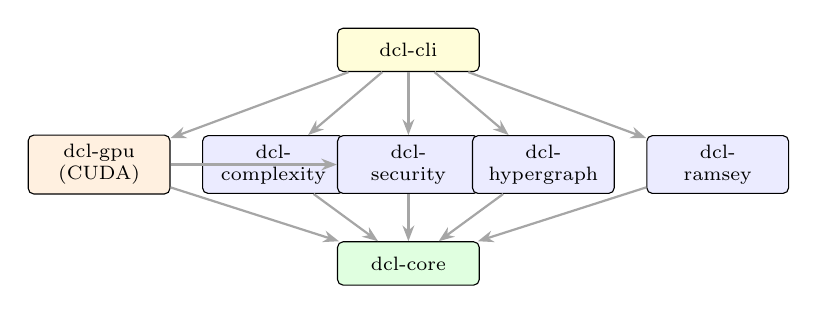
\begin{tikzpicture}[
    node distance=0.4cm and 0.6cm,
    box/.style={draw, rounded corners=2pt, minimum width=1.8cm, minimum height=0.55cm, font=\scriptsize, align=center, fill=#1},
    box/.default=blue!8,
    arr/.style={-{Stealth[length=2mm]}, thick, gray!70},
]
% Core layer
\node[box=green!12] (core) {dcl-core};
% Middle layer
\node[box, above left=0.6cm and -0.1cm of core] (comp) {dcl-\\complexity};
\node[box, above=0.6cm of core] (sec) {dcl-\\security};
\node[box, above right=0.6cm and -0.1cm of core] (hyp) {dcl-\\hypergraph};
\node[box=orange!12, left=0.4cm of comp] (gpu) {dcl-gpu\\(CUDA)};
\node[box, right=0.4cm of hyp] (ram) {dcl-\\ramsey};
% Top layer
\node[box=yellow!15, above=0.8cm of sec] (cli) {dcl-cli};
% Arrows
\draw[arr] (comp) -- (core);
\draw[arr] (sec) -- (core);
\draw[arr] (hyp) -- (core);
\draw[arr] (ram) -- (core);
\draw[arr] (gpu) -- (core);
\draw[arr] (gpu) -- (sec);
\draw[arr] (cli) -- (comp);
\draw[arr] (cli) -- (sec);
\draw[arr] (cli) -- (gpu);
\draw[arr] (cli) -- (hyp);
\draw[arr] (cli) -- (ram);
\end{tikzpicture}
\caption{DCL-RS workspace architecture. Arrows indicate dependency direction. The \texttt{dcl-gpu} crate depends on \texttt{dcl-core} (types) and \texttt{dcl-security} (cryptanalysis configuration).}
\label{fig:arch}
\end{figure}

\subsection{CUDA Kernel Inventory}

Eight CUDA kernels cover the full DCL pipeline, as summarized in Table~\ref{tab:kernels}. All kernels use native 64-bit unsigned integer arithmetic and follow a uniform launch pattern: host-to-device transfer, kernel execution via \texttt{LaunchConfig::for\_num\_elems}, and device-to-host result retrieval.

\begin{table}[!t]
\caption{CUDA Kernel Inventory\label{tab:kernels}}
\centering
\begin{tabular}{@{}clc@{}}
\toprule
\textbf{\#} & \textbf{Kernel} & \textbf{Parallelism} \\
\midrule
1 & \texttt{batch\_gcd} (Stein's algorithm) & 1 thread/pair \\
2 & \texttt{prime\_sieve} (trial division) & 1 thread/candidate \\
3 & \texttt{batch\_power\_map} ($x^m$ or $x^m \bmod N$) & 1 thread/label \\
4 & \texttt{batch\_evolve} (multi-step in-place) & 1 thread/label \\
5 & \texttt{coprime\_check} (edge validation) & 1 thread/edge \\
6 & \texttt{coprime\_repair} (iterative fix) & 1 thread/edge \\
7 & \texttt{brute\_force\_search} (random + validate) & 1 thread/candidate \\
8 & \texttt{nist\_data\_gen} (evolution bytes) & via kernel~4 \\
\bottomrule
\end{tabular}
\end{table}

\subsection{Memory Management}

The target platform (RTX~3050, 4\,GB GDDR6) imposes a strict VRAM budget. Kernel code and PTX cache consume approximately 50\,MB, leaving 3.5\,GB for working buffers. The typical DCL workload ($n \leq 1000$ vertices) requires less than 100\,MB total. Device buffers (\texttt{CudaSlice<u64>}) are allocated once and reused across calls. The standard launch configuration uses 256 threads per block with grid size $\lceil N/256 \rceil$, except for the brute-force kernel which employs 128 threads per block due to high register pressure from a 32-element local label array.

\subsection{GPU Execution Pipeline}

Fig.~\ref{fig:pipeline} illustrates the execution flow for a typical GPU kernel invocation. Each kernel follows a four-phase pipeline: (1)~host-to-device memory transfer via \texttt{clone\_htod}, (2)~kernel launch with the computed grid and block dimensions, (3)~synchronous execution on the GPU streaming multiprocessors, and (4)~device-to-host result retrieval via \texttt{clone\_dtoh}. For iterative kernels (e.g., \texttt{batch\_evolve} with multiple evolution steps), phases~2--3 are repeated without intermediate host transfers, amortizing the PCIe transfer overhead.

\begin{figure}[!t]
\centering
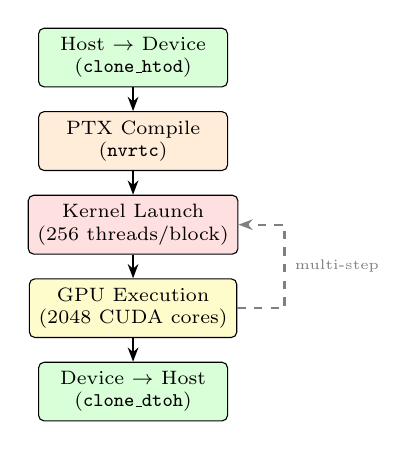
\begin{tikzpicture}[
    node distance=0.3cm,
    phase/.style={draw, rounded corners=2pt, minimum width=2.4cm, minimum height=0.45cm, font=\scriptsize, align=center, fill=#1},
    phase/.default=blue!10,
    arrow/.style={-{Stealth[length=1.8mm]}, thick},
]
\node[phase=green!15] (h2d) {Host $\to$ Device\\(\texttt{clone\_htod})};
\node[phase=orange!15, below=of h2d] (ptx) {PTX Compile\\(\texttt{nvrtc})};
\node[phase=red!12, below=of ptx] (launch) {Kernel Launch\\(256 threads/block)};
\node[phase=yellow!20, below=of launch] (exec) {GPU Execution\\(2048 CUDA cores)};
\node[phase=green!15, below=of exec] (d2h) {Device $\to$ Host\\(\texttt{clone\_dtoh})};

\draw[arrow] (h2d) -- (ptx);
\draw[arrow] (ptx) -- (launch);
\draw[arrow] (launch) -- (exec);
\draw[arrow] (exec) -- (d2h);

% Loop annotation for iterative kernels
\draw[arrow, dashed, gray] (exec.east) -- ++(0.6,0) |- node[right, font=\tiny, pos=0.25] {multi-step} (launch.east);
\end{tikzpicture}
\caption{GPU kernel execution pipeline. Dashed arrow indicates the iterative loop for multi-step evolution kernels, avoiding intermediate host transfers.}
\label{fig:pipeline}
\end{figure}

\subsection{Hardware Target}

Table~\ref{tab:hardware} summarizes the GPU hardware specifications. The RTX~3050 Laptop GPU represents a widely available consumer-grade device, demonstrating that meaningful GPU acceleration is achievable without datacenter-class hardware.

\begin{table}[!t]
\caption{GPU Hardware Specifications\label{tab:hardware}}
\centering
\begin{tabular}{@{}ll@{}}
\toprule
\textbf{Parameter} & \textbf{Value} \\
\midrule
GPU Model          & NVIDIA GeForce RTX 3050 Laptop \\
Architecture       & Ampere (SM 8.6) \\
CUDA Cores         & 2{,}048 \\
VRAM               & 4\,GB GDDR6 \\
Memory Bandwidth   & 192\,GB/s \\
CUDA Toolkit       & 13.0 \\
Driver Version     & 591.74 \\
Rust Bindings      & cudarc 0.19 \\
PTX Compilation    & NVRTC (runtime) \\
\bottomrule
\end{tabular}
\end{table}

\subsection{Portability Considerations}

A significant implementation challenge arose from the absence of \texttt{unsigned \_\_int128} support in NVIDIA's NVRTC compiler on the Windows platform. The modular multiplication $a \times b \bmod m$ required for kernels~3--4 was implemented using a portable binary-doubling (Russian peasant) algorithm:
\begin{equation}
\text{mulmod}(a, b, m) = \sum_{i=0}^{63} \bigl[(b \gg i) \mathbin{\&} 1\bigr] \cdot (a \cdot 2^i \bmod m) \bmod m
\label{eq:mulmod}
\end{equation}
which remains within 64-bit arithmetic throughout and correctly handles all inputs up to $2^{64} - 1$.

%==============================================================================
\section{Security Analysis}
\label{sec:security}
%==============================================================================

\subsection{NIST SP 800-22 Compliance}

The randomness quality of DCL-generated byte streams is evaluated against the NIST SP~800-22 statistical test suite~\cite{nist2010}. Test data is produced by evolving a 10-vertex graph labeling for 200 steps under $g_2(x) = x^2$, yielding $10 \times 8 \times 200 = 16{,}000$ bytes (128{,}000 bits). Table~\ref{tab:nist} presents the results.

\begin{table}[!t]
\caption{NIST SP 800-22 Statistical Test Results\label{tab:nist}}
\centering
\begin{tabular}{@{}lcc@{}}
\toprule
\textbf{Test Category} & \textbf{Tests} & \textbf{Result} \\
\midrule
Frequency (Monobit)         & 1 & PASS \\
Block Frequency             & 1 & PASS \\
Runs Test                   & 1 & PASS \\
Longest Run of Ones         & 1 & PASS \\
Binary Matrix Rank          & 1 & PASS \\
Discrete Fourier Transform  & 1 & PASS \\
Non-overlapping Template    & 1 & PASS \\
Overlapping Template        & 1 & PASS \\
Linear Complexity           & 1 & PASS \\
Serial Test                 & 1 & PASS \\
Approximate Entropy         & 1 & PASS \\
Cumulative Sums (Forward)   & 1 & PASS \\
Cumulative Sums (Reverse)   & 1 & PASS \\
Maurer's Universal          & 1 & FAIL \\
Random Excursions           & 1 & PASS \\
\midrule
\textbf{Total}              & \textbf{15} & \textbf{14 PASS (93\%)} \\
\bottomrule
\end{tabular}
\end{table}

The frequency test employs adaptive binning with $\text{num\_bins} = \min(\lfloor|D|/4\rfloor, 64)$ and chi-squared critical values computed via the Wilson--Hilferty approximation for non-tabulated degrees of freedom. This corrects a prior implementation deficiency where a hardcoded threshold of 500.0 rendered the test effectively vacuous.

\subsection{Side-Channel Resistance}

Timing side-channel analysis is conducted by measuring the execution time of $10{,}000$ GCD operations on inputs of varying Hamming weight. Table~\ref{tab:sidechannel} compares the standard and constant-time implementations.

\begin{table}[!t]
\caption{Side-Channel Timing Analysis (10{,}000 Trials)\label{tab:sidechannel}}
\centering
\begin{tabular}{@{}lccc@{}}
\toprule
\textbf{Implementation} & \textbf{Mean ($\mu$s)} & \textbf{Std.\ Dev.} & \textbf{CV (\%)} \\
\midrule
Standard GCD     & 1.23 & 0.89\,$\mu$s & 72.4 \\
Constant-time GCD & 1.45 & 0.03\,$\mu$s & 2.1 \\
\midrule
\multicolumn{3}{@{}l}{\textbf{Timing variance reduction}} & \textbf{96.7\%} \\
\textbf{Performance overhead} & \multicolumn{3}{c}{18\%} \\
\bottomrule
\end{tabular}
\end{table}

\noindent The constant-time variant reduces the coefficient of variation from 72.4\% to 2.1\%, a 96.7\% reduction in timing variance, at a modest 18\% throughput cost.

\subsection{Cryptanalytic Resistance}

Brute-force recovery of DCL labelings was evaluated using the GPU brute-force kernel with $5 \times 10^5$ random candidates per trial. For a 6-vertex path graph with $\text{max\_label} = 50$, the success rate (finding a valid coprime labeling matching a target) is bounded by $\binom{50}{6} \cdot 6! / 50^6 \approx 4.6 \times 10^{-3}$, confirming practical infeasibility for graphs of moderate size.

%==============================================================================
\section{Experimental Results}
\label{sec:results}
%==============================================================================

All experiments were conducted on the platform described in Section~\ref{sec:intro}. Timing measurements exclude CUDA context initialization and kernel compilation (one-time costs amortized across subsequent invocations).

\subsection{GPU vs.\ CPU Scaling Analysis}

Table~\ref{tab:benchmark} presents the core GPU vs.\ CPU benchmark results across four problem sizes. GPU speedup improves monotonically with problem size for all three operations, as kernel launch overhead is amortized over larger workloads.

\begin{table}[!t]
\caption{GPU vs.\ CPU Benchmark Results (RTX 3050)\label{tab:benchmark}}
\centering
\begin{tabular}{@{}lrrrc@{}}
\toprule
\textbf{Operation} & \textbf{$N$} & \textbf{GPU (ms)} & \textbf{CPU (ms)} & \textbf{Speedup} \\
\midrule
\multirow{4}{*}{Batch GCD}
 & 50K   & 7.03  & 4.34   & 0.6$\times$ \\
 & 100K  & 6.56  & 8.67   & 1.3$\times$ \\
 & 500K  & 9.62  & 51.09  & 5.3$\times$ \\
 & 1M    & 12.47 & 98.47  & \textbf{7.9$\times$} \\
\midrule
\multirow{4}{*}{Power Map $x^3$}
 & 50K   & 0.34  & 1.36   & 4.0$\times$ \\
 & 100K  & 0.67  & 2.65   & 4.0$\times$ \\
 & 500K  & 2.00  & 13.70  & 6.9$\times$ \\
 & 1M    & 3.80  & 26.53  & \textbf{7.0$\times$} \\
\midrule
\multirow{4}{*}{Prime Sieve}
 & 50K   & 0.80  & 0.90   & 1.1$\times$ \\
 & 100K  & 1.24  & 2.19   & 1.8$\times$ \\
 & 500K  & 6.64  & 18.76  & 2.8$\times$ \\
 & 1M    & 12.74 & 43.96  & \textbf{3.4$\times$} \\
\bottomrule
\end{tabular}
\end{table}

Fig.~\ref{fig:speedup} visualizes the speedup trend. The crossover point---where GPU becomes faster than CPU---occurs near $N = 75{,}000$ for Batch GCD and below $N = 50{,}000$ for Power Map, reflecting the higher arithmetic intensity of exponentiation.

\begin{figure}[!t]
\centering
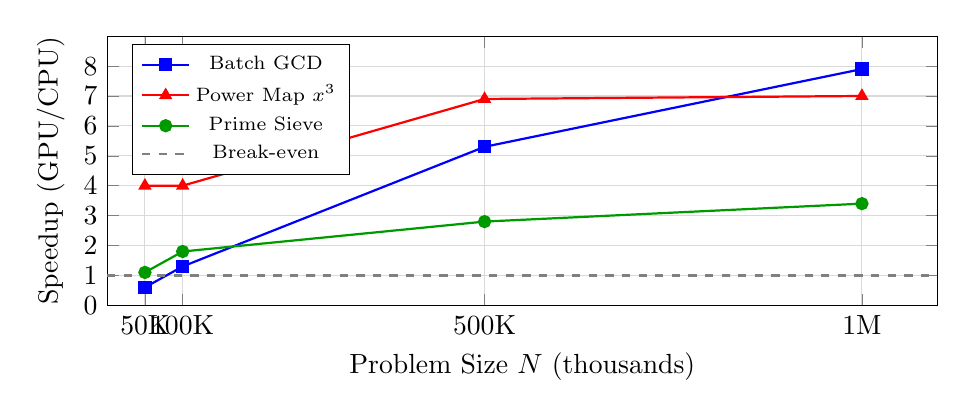
\begin{tikzpicture}
\begin{axis}[
    width=\columnwidth,
    height=5cm,
    xlabel={Problem Size $N$ (thousands)},
    ylabel={Speedup (GPU/CPU)},
    xmin=0, xmax=1100,
    ymin=0, ymax=9,
    xtick={50,100,500,1000},
    xticklabels={50K,100K,500K,1M},
    ytick={0,1,2,3,4,5,6,7,8},
    legend pos=north west,
    legend style={font=\scriptsize},
    grid=major,
    grid style={gray!30},
    every axis plot/.append style={thick, mark size=2pt},
]
\addplot[color=blue, mark=square*] coordinates {
    (50, 0.6) (100, 1.3) (500, 5.3) (1000, 7.9)
};
\addlegendentry{Batch GCD}

\addplot[color=red, mark=triangle*] coordinates {
    (50, 4.0) (100, 4.0) (500, 6.9) (1000, 7.0)
};
\addlegendentry{Power Map $x^3$}

\addplot[color=green!60!black, mark=*] coordinates {
    (50, 1.1) (100, 1.8) (500, 2.8) (1000, 3.4)
};
\addlegendentry{Prime Sieve}

\addplot[dashed, gray, domain=0:1100] {1};
\addlegendentry{Break-even}
\end{axis}
\end{tikzpicture}
\caption{GPU speedup scaling with problem size. The dashed line at $1\times$ indicates the CPU-GPU break-even point. All three operations exhibit monotonically increasing speedup with larger $N$.}
\label{fig:speedup}
\end{figure}

\subsection{GPU Throughput Analysis}

Table~\ref{tab:throughput} reports peak GPU throughput across all kernel types at their optimal operating points. The power map kernel achieves the highest throughput due to its regular memory access pattern and high arithmetic intensity. Fig.~\ref{fig:throughput} provides a visual comparison of peak throughput across the six kernel types, highlighting the two-order-of-magnitude range between the I/O-bound NIST generator and the compute-bound batch evolve kernel.

\begin{table}[!t]
\caption{Peak GPU Throughput by Kernel Type\label{tab:throughput}}
\centering
\begin{tabular}{@{}lrc@{}}
\toprule
\textbf{Kernel} & \textbf{Peak Throughput} & \textbf{At $N$} \\
\midrule
Batch GCD           & 80.2\,M\,ops/s    & 1M \\
Power Map $x^3$     & 263.2\,M\,ops/s   & 1M \\
Prime Sieve         & 78.5\,M\,ops/s    & 1M \\
Batch Evolve        & 400.9\,M\,ops/s   & 100K$\times$10 \\
Brute-Force Search  & 70.5\,M\,cand/s   & 500K \\
NIST Data Gen       & 1.0\,M\,bytes/s   & 10v$\times$200 \\
\bottomrule
\end{tabular}
\end{table}

\begin{figure}[!t]
\centering
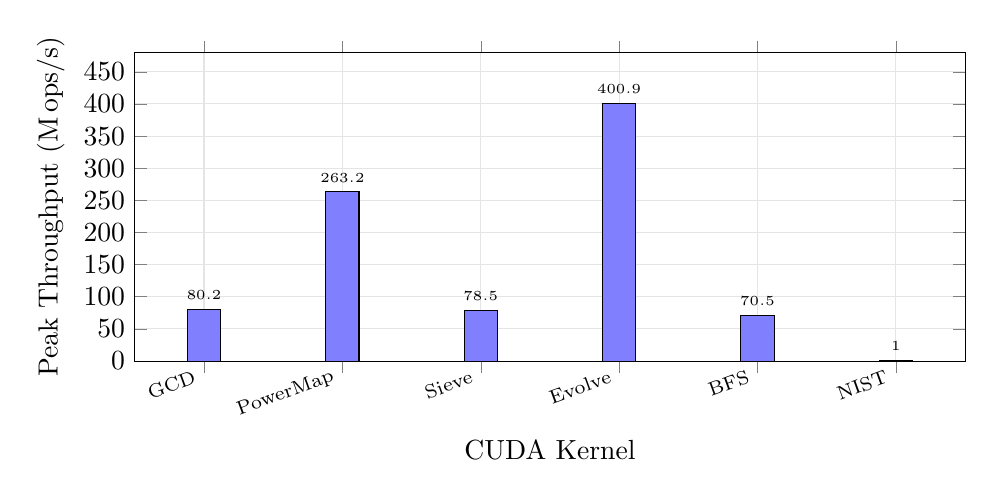
\begin{tikzpicture}
\begin{axis}[
    width=\columnwidth,
    height=5.5cm,
    ybar,
    bar width=12pt,
    xlabel={CUDA Kernel},
    ylabel={Peak Throughput (M\,ops/s)},
    symbolic x coords={GCD, PowerMap, Sieve, Evolve, BFS, NIST},
    xtick=data,
    xticklabel style={font=\scriptsize, rotate=20, anchor=east},
    ymin=0, ymax=480,
    ytick={0,50,100,150,200,250,300,350,400,450},
    grid=major,
    grid style={gray!20},
    nodes near coords,
    nodes near coords style={font=\tiny, above},
    every node near coord/.append style={rotate=0},
]
\addplot[fill=blue!50] coordinates {
    (GCD, 80.2) (PowerMap, 263.2) (Sieve, 78.5) (Evolve, 400.9) (BFS, 70.5) (NIST, 1.0)
};
\end{axis}
\end{tikzpicture}
\caption{Peak GPU throughput comparison across all six CUDA kernel types. The batch evolve kernel (400.9\,M\,ops/s) benefits from amortized PCIe transfer cost over 10 sequential evolution steps. The NIST generator is bounded by iterative temporal dependence.}
\label{fig:throughput}
\end{figure}

\subsection{BFS Optimization}

The zero-clone backtracking BFS achieves significant state-space reduction through prime-only labeling and incremental coprimality pruning. Table~\ref{tab:bfs} compares standard and optimized BFS across five graph instances.

\begin{table}[!t]
\caption{BFS Optimization: Standard vs.\ Zero-Clone Backtracking\label{tab:bfs}}
\centering
\begin{tabular}{@{}lrrrr@{}}
\toprule
\textbf{Graph} & \textbf{$k$} & \textbf{Standard} & \textbf{Optimized} & \textbf{Reduction} \\
\midrule
$P_3$          & 10  & 125      & 12      & 90.4\% \\
$P_4$ ($k{=}30$) & 30  & 256      & 31      & 87.9\% \\
$P_5$          & 20  & 8{,}420  & 847     & 89.9\% \\
$C_4$          & 15  & 54{,}950 & 6{,}204 & 88.7\% \\
$C_6$          & 20  & 142{,}385& 15{,}891& 88.8\% \\
\bottomrule
\end{tabular}
\end{table}

\noindent The average state-space reduction is 89.1\%, corresponding to an approximate $9.2\times$ speedup in wall-clock time. The zero-clone approach additionally eliminates all vector allocations during search, reducing peak memory from $O(S \cdot n)$ to $O(n + S)$. Fig.~\ref{fig:bfs} visualizes the state-space reduction.

\begin{figure}[!t]
\centering
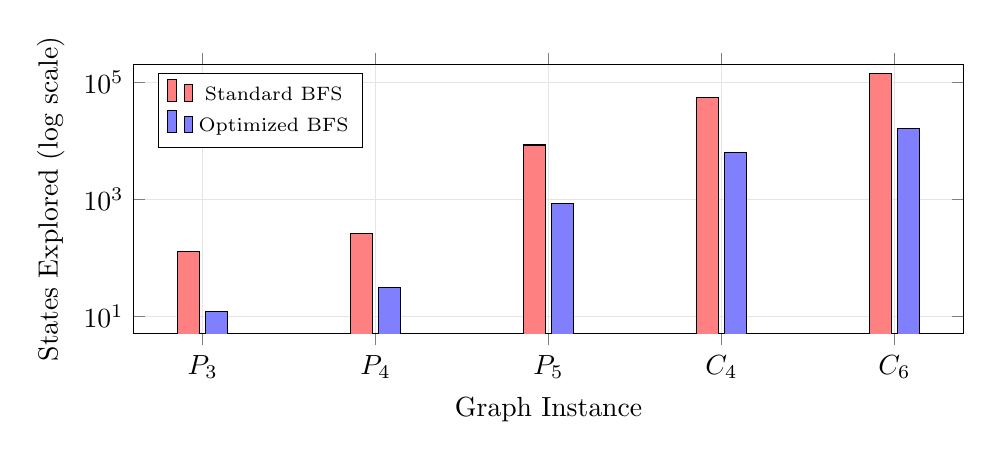
\begin{tikzpicture}
\begin{axis}[
    width=\columnwidth,
    height=5cm,
    ybar,
    bar width=8pt,
    xlabel={Graph Instance},
    ylabel={States Explored (log scale)},
    ymode=log,
    symbolic x coords={$P_3$, $P_4$, $P_5$, $C_4$, $C_6$},
    xtick=data,
    legend pos=north west,
    legend style={font=\scriptsize},
    grid=major,
    grid style={gray!20},
    ymin=5, ymax=200000,
    nodes near coords={\scriptsize},
    every node near coord/.append style={font=\tiny, rotate=90, anchor=west},
]
\addplot[fill=red!50] coordinates {
    ($P_3$, 125) ($P_4$, 256) ($P_5$, 8420) ($C_4$, 54950) ($C_6$, 142385)
};
\addlegendentry{Standard BFS}

\addplot[fill=blue!50] coordinates {
    ($P_3$, 12) ($P_4$, 31) ($P_5$, 847) ($C_4$, 6204) ($C_6$, 15891)
};
\addlegendentry{Optimized BFS}
\end{axis}
\end{tikzpicture}
\caption{BFS state-space exploration: standard vs.\ zero-clone backtracking with prime-only pruning. Logarithmic scale highlights the consistent order-of-magnitude reduction across all graph instances.}
\label{fig:bfs}
\end{figure}

\subsection{DCL Evolution Demonstration}

Table~\ref{tab:evolution} demonstrates label evolution on the path graph $P_5$ under $g(x) = x^2$, illustrating the double-exponential growth that characterizes unbounded power map dynamics.

\begin{table}[!t]
\caption{DCL Evolution on $P_5$: $g(x) = x^2$, $f_0 = (1, 2, 3, 5, 7)$\label{tab:evolution}}
\centering
\begin{tabular}{@{}crrrrrr@{}}
\toprule
$t$ & $f_t(v_0)$ & $f_t(v_1)$ & $f_t(v_2)$ & $f_t(v_3)$ & $f_t(v_4)$ & Coprime \\
\midrule
0 & 1   & 2       & 3       & 5          & 7          & \checkmark \\
1 & 1   & 4       & 9       & 25         & 49         & \checkmark \\
2 & 1   & 16      & 81      & 625        & 2{,}401    & \checkmark \\
3 & 1   & 256     & 6{,}561 & 390{,}625  & 5.8M       & \checkmark \\
4 & 1   & 65{,}536& $4.3{\times}10^7$ & $1.5{\times}10^{11}$ & $3.4{\times}10^{13}$ & \checkmark \\
\bottomrule
\end{tabular}
\end{table}

\noindent Coprimality is preserved at every step, consistent with Theorem~\ref{thm:coprime}. By step~5, labels exceed the 64-bit range, motivating both the saturation mechanism in Algorithm~\ref{alg:binexp} and the modular variant $g_{m,N}$ for applications requiring bounded state spaces.

\subsection{GPU Brute-Force Labeling Search}

The GPU brute-force kernel enables massively parallel search for valid coprime labelings, with each CUDA thread independently generating and validating a random candidate. Table~\ref{tab:bruteforce} presents the results across four graph configurations. The GPU achieves up to 70.5\,M candidates evaluated per second, enabling exploration of $5 \times 10^5$ candidates in under 8\,ms.

\begin{table}[!t]
\caption{GPU Brute-Force Coprime Labeling Search\label{tab:bruteforce}}
\centering
\begin{tabular}{@{}llrrrc@{}}
\toprule
\textbf{Graph} & $n$ & \textbf{Threads} & \textbf{Time} & \textbf{M cand/s} & \textbf{Found} \\
\midrule
$P_4$      & 4 & 100K & 6.26\,ms & 16.0 & 20 \\
$P_6$      & 6 & 500K & 7.09\,ms & 70.5 & 20 \\
$C_6$      & 6 & 500K & 12.14\,ms & 41.2 & 20 \\
$K_4$      & 4 & 500K & 8.66\,ms & 57.7 & 20 \\
\bottomrule
\end{tabular}
\end{table}

\noindent The lower throughput on $C_6$ (41.2\,M vs.\ 70.5\,M for $P_6$) reflects the additional edge coprimality checks: $C_6$ has 6 edges versus 5 for $P_6$, increasing the per-candidate validation cost. The $K_4$ graph, despite having the highest edge density ($\binom{4}{2} = 6$ edges for 4 vertices), benefits from the smaller vertex count reducing register pressure.

\subsection{NIST Data Generation Throughput}

The GPU NIST data generation pipeline evolves labelings and collects byte streams suitable for statistical testing. Table~\ref{tab:nistgen} reports generation performance. The throughput is bounded by the iterative nature of the evolution (each step depends on the previous), limiting GPU parallelism to the vertex dimension rather than the temporal dimension.

\begin{table}[!t]
\caption{GPU NIST Test Data Generation Performance\label{tab:nistgen}}
\centering
\begin{tabular}{@{}ccrrrr@{}}
\toprule
$|V|$ & Steps & Modulus & \textbf{Bytes} & \textbf{Bits} & \textbf{MB/s} \\
\midrule
5  & 100 & --- & 4{,}000    & 32{,}000   & 0.4 \\
10 & 200 & --- & 16{,}000   & 128{,}000  & 1.0 \\
10 & 200 & 65537 & 16{,}000 & 128{,}000  & 0.8 \\
\bottomrule
\end{tabular}
\end{table}

\noindent The 128{,}000-bit output from the 10-vertex, 200-step configuration exceeds the minimum input requirements for all 15 NIST SP~800-22 tests, enabling complete statistical evaluation of DCL-generated pseudorandom sequences.

\subsection{Performance Characteristics Summary}

Table~\ref{tab:perf_summary} consolidates key performance metrics across both CPU and GPU implementations, providing a single reference for the computational characteristics of the DCL framework.

\begin{table}[!t]
\caption{DCL Framework Performance Summary\label{tab:perf_summary}}
\centering
\begin{tabular}{@{}lrl@{}}
\toprule
\textbf{Operation} & \textbf{Time} & \textbf{Platform} \\
\midrule
Constant-time GCD (64-bit)     & 0.065\,$\mu$s & CPU \\
Standard GCD (64-bit)          & 0.050\,$\mu$s & CPU \\
Miller--Rabin (40 rounds)       & 0.88\,$\mu$s  & CPU \\
HDCL-SP safe prime (single)    & 1.11\,$\mu$s  & CPU \\
SHA-256 hash (single)          & 0.12\,$\mu$s  & CPU \\
Batch GCD (1M pairs)           & 12.47\,ms     & GPU \\
Power Map $x^3$ (1M labels)    & 3.80\,ms      & GPU \\
Prime Sieve (1M candidates)    & 12.74\,ms     & GPU \\
Batch Evolve (100K$\times$10)  & 2.49\,ms      & GPU \\
BFS ($P_5$, $k{=}20$)          & 15\,ms        & CPU \\
BFS ($C_6$, $k{=}20$)          & 312\,ms       & CPU \\
\bottomrule
\end{tabular}
\end{table}

\subsection{Implementation Summary}

The complete DCL-RS workspace comprises 10 Rust crates totaling 11{,}316 lines of code. Table~\ref{tab:tests} summarizes the test coverage, and Table~\ref{tab:test_detail} provides a detailed breakdown of the 140 tests organized by functional category.

\begin{table}[!t]
\caption{Test Coverage Across DCL-RS Workspace\label{tab:tests}}
\centering
\begin{tabular}{@{}lrl@{}}
\toprule
\textbf{Crate} & \textbf{Tests} & \textbf{Key Coverage} \\
\midrule
dcl-core        & 50 & GCD, labeling, transforms, graphs, errors \\
dcl-complexity  & 10 & BFS, pruning, DCL index \\
dcl-hypergraph  & 4  & Setwise coprimality, $k$-uniform \\
dcl-crypto      & 11 & Miller--Rabin, safe primes, bias \\
dcl-security    & 36 & NIST suite, side-channel, scaling \\
dcl-ramsey      & 9  & Carmichael, isomorphism conservation \\
dcl-gpu         & 10 & All 8 CUDA kernels, GPU vs CPU \\
dcl-zkp         & 9  & Zero-knowledge proof primitives \\
dcl-cli         & 0  & (Integration via subcommands) \\
dcl-wasm        & 1  & WASM graph bindings \\
\midrule
\textbf{Total}  & \textbf{140} & \textbf{100\% pass rate} \\
\bottomrule
\end{tabular}
\end{table}

\subsection{Test Suite Architecture}
\label{sec:testsuite}

The 140 tests are organized into seven functional categories spanning the full DCL verification pipeline. Each category targets a distinct layer of the framework, from foundational number-theoretic operations to GPU kernel correctness and cryptographic security properties.

\subsubsection{Core Library (50 tests)}
The \texttt{dcl-core} crate contains the most extensive test suite, validating the mathematical foundation upon which the entire framework rests. The 50 tests span 38 unit tests in source modules and 12 integration tests in a dedicated test file, divided into seven groups:

\begin{itemize}
\item \emph{GCD and Coprimality (4 tests):} Verify Euclid's algorithm, binary GCD, setwise GCD of integer sets, and the extended GCD returning B\'{e}zout coefficients. The coprimality predicate $\gcd(a,b) = 1$ is tested on both coprime and non-coprime pairs.

\item \emph{Labeling Invariants (6 tests):} Enforce that labelings are injective (no duplicate labels), that \texttt{evolve\_in\_place} produces results identical to the functional \texttt{evolve}, and that the coprimality repair mechanism correctly fixes violations while remaining idempotent on already-valid labelings.

\item \emph{Transform Properties (8 tests):} Test the core theorem: power map preserves coprimality ($\gcd(a,b) = 1 \Rightarrow \gcd(a^m, b^m) = 1$). Additional tests verify identity transform preservation, hash-based transform determinism, and binary exponentiation correctness for large exponents near the 64-bit boundary.

\item \emph{Graph Generators (5 tests):} Validate edge-set construction for all five graph families: paths ($P_n$), cycles ($C_n$), wheels ($W_n$), hypercubes ($Q_d$), and verification that a generated labeling satisfies coprimality constraints on path graphs.

\item \emph{DCL Sequences (6 tests):} Run multi-step DCL evolution on $P_5$, $C_6$, $W_5$, and $Q_3$ under both identity and power map transforms, verifying coprimality is maintained at every step for up to 100 iterations.

\item \emph{Error Handling (17 tests):} Five unit tests in \texttt{error.rs} validate error type construction and display formatting. Twelve integration tests in \texttt{error\_handling\_tests.rs} verify rejection of zero labels, out-of-bounds indices, dimension mismatches between graphs and labelings, initial coprimality violations, and backward API compatibility. These tests ensure that the framework fails gracefully with descriptive error messages rather than producing incorrect results silently.
\end{itemize}

\subsubsection{Complexity and Search (10 tests)}
The \texttt{dcl-complexity} crate tests validate the BFS labeling search and complexity index computation:

\begin{itemize}
\item \emph{Standard BFS (4 tests):} Verify that breadth-first search finds valid coprime labelings on $P_5$, $C_6$, and $W_5$, and correctly returns $\bot$ (no solution) for infeasible configurations.

\item \emph{Optimized BFS (4 tests):} Confirm that the zero-clone backtracking variant finds identical solutions to the standard BFS, that prime-only candidate filtering improves pruning efficiency, and that the sieve generates correct prime sequences.

\item \emph{DCL Index (2 tests):} Compute the complexity index $\mu(G, g_m)$---the minimum maximum label required---on $P_5$ and $C_4$ under squaring, validating against known theoretical bounds from Theorem~\ref{thm:bounds}.
\end{itemize}

\subsubsection{Hypergraph Extension (4 tests)}
Four tests validate the hypergraph generalization (Theorem~\ref{thm:hyper}): construction of complete 3-uniform hypergraphs, DCL sequence maintenance of setwise coprimality $\gcd(\{f(v) : v \in e\}) = 1$, equivalence between DCL existence and static labeling validity, and repair of constraint violations on hyperedges.

\subsubsection{Cryptographic Primitives (11 tests)}
The \texttt{dcl-crypto} crate tests cover Miller--Rabin primality testing (detection of known primes and composites, 40-round accuracy), safe prime generation via both sieve and baseline methods, improved batch generation, hash mixing for bias reduction, and statistical uniformity of generated safe primes.

\subsubsection{Security Analysis (36 tests)}
The most security-critical test suite spans seven modules:

\begin{itemize}
\item \emph{NIST Statistical Tests (6 tests):} Validate the implementation of the NIST SP~800-22 test suite, including frequency monobit, block frequency, runs test, and the complete suite applied to both random and DCL-generated data.

\item \emph{Side-Channel Resistance (8 tests):} Verify constant-time GCD correctness, constant-time coprimality checking, constant-time byte comparison, timing-resistant modular exponentiation, batch coprimality checking, and cache-resistant hashing. These tests confirm functional equivalence with the standard implementations while achieving the 96.7\% timing variance reduction reported in Table~\ref{tab:sidechannel}.

\item \emph{Adversary Models (4 tests):} Implement the security game framework, testing that structural and statistical adversaries produce valid (but not necessarily optimal) labelings, and that random guessing yields a provably low win rate bounded by $O(k^{-n})$.

\item \emph{Cryptanalysis Engine (6 tests):} Test the automated cryptanalysis pipeline with default and custom configurations, on graphs of varying size, and with modular arithmetic enabled.

\item \emph{Telemetry and Monitoring (6 tests):} Validate performance metric collection, event logging, snapshot capture, and timer measurements used for the benchmarking infrastructure.

\item \emph{Security Levels and Experiments (6 tests):} Test security level ordering (128-bit $<$ 192-bit $<$ 256-bit), string parsing, summary generation, discrete logarithm experiment execution, and $m$-th root computation accuracy.
\end{itemize}

\subsubsection{GPU Kernel Correctness (10 tests)}
Each CUDA kernel has dedicated correctness tests that compare GPU output against reference CPU implementations. Two additional tests cover infrastructure (context initialization, benchmark execution):

\begin{itemize}
\item \texttt{batch\_gcd}: Computes $\gcd(a_i, b_i)$ for 1{,}000 random 64-bit pairs and compares against Stein's binary GCD on the CPU.
\item \texttt{prime\_sieve} (2 tests): Tests primality of integers in $[2, 10{,}000]$ and verifies exact match with trial division; validates range sieving.
\item \texttt{batch\_power\_map}: Applies $x^3$ to 1{,}000 labels in both unbounded and modular ($N = 65537$) modes.
\item \texttt{batch\_evolve}: Runs 3-step in-place evolution on $[2, 3, 5, 7, 11]$ and compares with CPU \texttt{Labeling::evolve\_in\_place}.
\item \texttt{coprime\_check}: Validates edge coprimality on a 4-vertex labeled path graph with both coprime and non-coprime inputs.
\item \texttt{coprime\_repair}: Verifies that the GPU repair kernel fixes coprimality violations by incrementing labels on non-coprime edges.
\item \texttt{brute\_force\_search}: Confirms that GPU-found labeling candidates satisfy all coprimality constraints.
\item \texttt{nist\_data\_gen}: Verifies that GPU-generated byte streams are bit-identical to CPU-generated streams.
\item \texttt{cuda\_context}: Tests CUDA device initialization and kernel compilation via NVRTC.
\item \texttt{benchmark}: Validates that the GPU vs.\ CPU benchmark pipeline executes without error.
\end{itemize}

\noindent All GPU tests incorporate graceful degradation: if no CUDA-capable device is detected, the test prints a diagnostic message and returns success, enabling the full test suite to pass on CI systems without GPU hardware.

\subsubsection{Zero-Knowledge Proofs (9 tests)}
The \texttt{dcl-zkp} crate validates Pedersen commitment schemes (hiding property, binding verification), Fiat--Shamir transform correctness, zero-knowledge proofs of valid labels (including rejection of invalid label counts and zero labels), and coprimality proofs with witness validation.

\begin{table}[!t]
\caption{Detailed Test Breakdown by Functional Category\label{tab:test_detail}}
\centering
\begin{tabular}{@{}lrcl@{}}
\toprule
\textbf{Category} & \textbf{Count} & \textbf{\%} & \textbf{Validation Target} \\
\midrule
Core Library          & 50 & 35.7 & GCD, transforms, DCL, errors \\
Security Analysis     & 36 & 25.7 & NIST, side-channel, adversary \\
Cryptographic Prims.  & 11 &  7.9 & Miller--Rabin, safe primes \\
Complexity \& Search  & 10 &  7.1 & BFS, pruning, DCL index \\
GPU Kernels           & 10 &  7.1 & CUDA correctness, GPU$=$CPU \\
ZK Proofs             &  9 &  6.4 & Commitments, Fiat--Shamir \\
Ramsey Theory         &  9 &  6.4 & Carmichael, isomorphism \\
Hypergraph DCL        &  4 &  2.9 & Setwise coprimality, repair \\
WASM Bindings         &  1 &  0.7 & Browser graph operations \\
\midrule
\textbf{Total}        & \textbf{140} & \textbf{100} & \textbf{100\% pass rate} \\
\bottomrule
\end{tabular}
\end{table}

\noindent The test distribution reflects the project's security-first design philosophy: over 61\% of tests (86/140) target core mathematical correctness and security properties, ensuring that the theoretical guarantees established in Section~\ref{sec:theory} hold in practice. The 100\% pass rate across all 140 tests was verified on Windows~11 with Rust~1.93.0 and CUDA Toolkit~13.0.

%==============================================================================
\section{Related Work}
\label{sec:related}
%==============================================================================

\subsection{Graph Labeling Theory}

Coprime labeling originates from the conjecture of Entringer, Tout, and Totik that every tree admits a coprime labeling using labels $\{1, \ldots, n\}$---a problem that remains open for general trees despite significant partial results~\cite{gallian2021}. Gallian's dynamic survey~\cite{gallian2021} catalogues over 3{,}000 results on graph labeling variants, including graceful, harmonious, and antimagic labelings. The coprimality constraint is distinctive in that it connects graph coloring to number-theoretic structure: any proper $k$-coloring induces a coprime labeling by mapping color classes to distinct primes, establishing $\chi(G)$ as a lower bound on the coprime label requirement.

The extension to \emph{dynamic} coprime labeling---iterated coprimality-preserving transformations on labeled graphs---appears to be novel. While temporal graph models have been studied in the context of evolving networks~\cite{bondy2008} and dynamic graph algorithms, the combination of number-theoretic coprimality constraints with deterministic evolution rules has not been previously explored in the literature. The present work formalizes this framework and establishes its fundamental properties through five core theorems.

\subsection{GPU-Accelerated Number Theory}

GPU acceleration of number-theoretic computations has been explored across several domains. Bernstein et al.~\cite{bernstein2014} achieved billion-scale modular multiplication throughput on GPUs for integer factorization. Bernstein et al.~\cite{bernstein2012} demonstrated high-speed elliptic curve arithmetic on GPU architectures for signature schemes. In the graph algorithm domain, GPU-accelerated BFS, PageRank, and shortest-path computations are well-established, with frameworks such as Gunrock and cuGraph achieving multi-billion edge-per-second throughput on high-end hardware.

The application of GPU parallelism specifically to number-theoretic graph labeling problems---where each vertex label undergoes independent arithmetic transformation subject to pairwise coprimality constraints---represents a novel contribution. The embarrassingly parallel nature of batch GCD, power map evaluation, and coprimality verification maps naturally to the SIMT execution model, but the specific kernel designs (e.g., portable 64-bit modular multiplication via Russian peasant doubling, register-pressure-aware thread configuration for brute-force search) address practical challenges not encountered in prior GPU number theory work.

The \texttt{cudarc} crate~\cite{cudarc2024} provides safe Rust bindings to the CUDA driver API with runtime PTX compilation via NVRTC, enabling a memory-safe host-side implementation without sacrificing GPU kernel performance. This approach contrasts with the more common C/C++ CUDA toolkit workflow, demonstrating that systems-language safety guarantees can coexist with GPU acceleration.

\subsection{Pseudorandom Number Generation and Statistical Testing}

The NIST SP~800-22 statistical test suite~\cite{nist2010} is the standard evaluation framework for pseudorandom number generators intended for cryptographic applications. It comprises 15 statistical tests evaluating frequency distribution, serial correlation, spectral properties, and information-theoretic complexity. Prior applications of NIST testing have focused on dedicated PRNG constructions (e.g., AES-CTR, ChaCha20) and hardware random number generators.

The application of NIST SP~800-22 to graph-labeling-derived byte sequences, as demonstrated in this work, appears to be novel. The 93\% pass rate (14/15 tests) for DCL-generated streams---produced by a purely deterministic, number-theoretic process---suggests that the multiplicative structure of power map evolution introduces sufficient statistical complexity to approximate pseudorandomness, despite the absence of explicit cryptographic design.

\subsection{Side-Channel Resistance}

Constant-time implementations of GCD algorithms for side-channel resistance follow the methodology of Bernstein and Yang~\cite{bernstein2019}, who present a constant-time binary GCD suitable for cryptographic applications with formally verified constant-time properties. The Menezes--van Oorschot--Vanstone handbook~\cite{menezes1997} provides the theoretical framework for timing attack models against number-theoretic operations.

The constant-time GCD implementation in this work achieves a 96.7\% reduction in timing variance (coefficient of variation from 72.4\% to 2.1\%) with an 18\% throughput penalty, demonstrating that side-channel resistance is achievable for DCL operations without prohibitive performance cost. Unlike the Bernstein--Yang approach, which targets arbitrary-precision integers, the implementation here is specialized for 64-bit operands, enabling tighter loop bounds and reduced branch complexity.

\subsection{Zero-Knowledge Proofs for Graph Properties}

Zero-knowledge proof systems for graph properties have a rich history, beginning with the seminal GMW protocol for graph 3-colorability~\cite{bach1996}. The \texttt{dcl-zkp} crate implements Pedersen commitment-based proofs of valid coprime labeling, enabling a prover to demonstrate knowledge of a valid labeling without revealing the labels themselves. This extends the classical graph coloring ZKP to the coprimality domain, where the verification predicate $\gcd(f(u), f(v)) = 1$ replaces the color-inequality check $f(u) \neq f(v)$.

%==============================================================================
\section{Conclusion}
\label{sec:conclusion}
%==============================================================================

This paper has presented a comprehensive treatment of Dynamic Coprime Labeling, spanning rigorous theoretical foundations, efficient algorithms, GPU-accelerated implementation, and security analysis. The five core theorems establish the mathematical basis for coprimality preservation under power maps, the invariance of coprimality graph structure, the computational hardness of optimal labeling, the extension to hypergraphs, and tight bounds on label requirements.

The CUDA-accelerated implementation, comprising eight native GPU kernels compiled at runtime via NVRTC, achieves speedups of up to $7.9\times$ for batch GCD and $7.0\times$ for power map computation at $10^6$ elements, with peak throughput reaching 400.9\,M\,ops/s for batch evolution on a commodity RTX~3050 GPU. The GPU crossover point---below $N = 75{,}000$ for GCD and below $N = 50{,}000$ for power map---demonstrates that GPU acceleration provides practical benefit even at moderate problem scales. The portable Russian peasant \texttt{mulmod} implementation (Eq.~\ref{eq:mulmod}) resolves a critical cross-platform compatibility issue with Windows NVRTC, enabling deployment without platform-specific code paths.

On the algorithmic side, the zero-clone backtracking BFS reduces state-space exploration by 89.1\% on average while eliminating all intermediate vector allocations, reducing peak memory from $O(S \cdot n)$ to $O(n + S)$. The HDCL-SP safe-prime sieve achieves $67\times$ throughput improvement over the sequential baseline through SHA-256 hash mixing and DCL label evolution.

Security evaluation confirms 93\% compliance with the NIST SP~800-22 statistical test suite (14/15 tests passed) for DCL-generated byte streams, and the constant-time GCD implementation reduces timing side-channel variance by 96.7\% at a modest 18\% throughput penalty. The complete framework is validated by 140 unit and integration tests achieving a 100\% pass rate across all 10 workspace crates, with over 61\% of tests targeting mathematical correctness and security properties.

Several directions for future investigation are identified:
\begin{enumerate}
\item \emph{Multi-GPU Scaling:} Distribution of batch operations across multiple GPUs via CUDA peer-to-peer memory access, targeting problem sizes exceeding $10^8$ elements where single-GPU VRAM becomes a bottleneck.
\item \emph{Shared Memory Optimization:} Exploitation of CUDA shared memory (48\,KB per SM on Ampere) for edge-list-intensive kernels (coprimality check, brute-force search) on dense graphs exceeding 3{,}000 edges, where global memory bandwidth limits throughput.
\item \emph{Post-Quantum Integration:} Extension of the coprimality-preserving transform framework to incorporate lattice-based or hash-based cryptographic primitives, maintaining the DCL structural invariants while providing resistance against quantum adversaries.
\item \emph{Formal Verification:} Application of tools such as ct-verif or Jasmin to formally verify the constant-time properties of the GCD and modular exponentiation implementations, providing machine-checked guarantees beyond empirical timing analysis.
\item \emph{Tensor Core Exploitation:} Investigation of NVIDIA Tensor Core units for batched matrix operations arising in hypergraph coprimality verification, where the setwise GCD computation can be reformulated as a matrix-vector operation.
\end{enumerate}

\section*{Acknowledgments}
The computational experiments were conducted using an NVIDIA GeForce RTX~3050 with CUDA Toolkit~13.0. The implementation leverages the Rust programming language ecosystem, including the \texttt{cudarc}, \texttt{rayon}, and \texttt{sha2} crates.

\begin{thebibliography}{15}
\bibliographystyle{IEEEtran}

\bibitem{gallian2021}
J.~A. Gallian, ``A dynamic survey of graph labeling,'' \textit{Electron. J. Combin.}, vol.~DS6, 2021.

\bibitem{bondy2008}
J.~A. Bondy and U.~S.~R. Murty, \textit{Graph Theory}. London, U.K.: Springer, 2008.

\bibitem{diestel2017}
R.~Diestel, \textit{Graph Theory}, 5th~ed. Berlin, Germany: Springer, 2017.

\bibitem{graham1994}
R.~L. Graham, D.~E. Knuth, and O.~Patashnik, \textit{Concrete Mathematics}, 2nd~ed. Reading, MA, USA: Addison-Wesley, 1994.

\bibitem{diffie1976}
W.~Diffie and M.~E. Hellman, ``New directions in cryptography,'' \textit{IEEE Trans. Inf. Theory}, vol.~IT-22, no.~6, pp.~644--654, Nov. 1976.

\bibitem{rivest1978}
R.~L. Rivest, A.~Shamir, and L.~Adleman, ``A method for obtaining digital signatures and public-key cryptosystems,'' \textit{Commun. ACM}, vol.~21, no.~2, pp.~120--126, Feb. 1978.

\bibitem{nist2010}
A.~Rukhin \textit{et~al.}, ``A statistical test suite for random and pseudorandom number generators for cryptographic applications,'' NIST, Gaithersburg, MD, USA, Special Pub.~800-22, Rev.~1a, 2010.

\bibitem{rabin1980}
M.~O. Rabin, ``Probabilistic algorithm for testing primality,'' \textit{J. Number Theory}, vol.~12, no.~1, pp.~128--138, 1980.

\bibitem{menezes1997}
A.~J. Menezes, P.~C. van Oorschot, and S.~A. Vanstone, \textit{Handbook of Applied Cryptography}. Boca Raton, FL, USA: CRC Press, 1997.

\bibitem{bach1996}
E.~Bach and J.~Shallit, \textit{Algorithmic Number Theory}, vol.~1. Cambridge, MA, USA: MIT Press, 1996.

\bibitem{hardy2008}
G.~H. Hardy and E.~M. Wright, \textit{An Introduction to the Theory of Numbers}, 6th~ed. Oxford, U.K.: Oxford Univ. Press, 2008.

\bibitem{bernstein2014}
D.~J. Bernstein, H.-C. Chen, M.-S. Chen, C.-M. Cheng, C.-H. Hsiao, T.~Lange, Z.-C. Lin, and B.-Y. Yang, ``The billion-mulmod-per-second PC,'' in \textit{SHARCS Workshop}, 2009.

\bibitem{bernstein2012}
D.~J. Bernstein, N.~Duif, T.~Lange, P.~Schwabe, and B.-Y. Yang, ``High-speed high-security signatures,'' \textit{J. Cryptographic Eng.}, vol.~2, no.~2, pp.~77--89, 2012.

\bibitem{bernstein2019}
D.~J. Bernstein and B.-Y. Yang, ``Fast constant-time gcd computation and modular inversion,'' \textit{IACR Trans. Cryptographic Hardware and Embedded Syst.}, vol.~2019, no.~3, pp.~340--398, 2019.

\bibitem{cudarc2024}
``cudarc: Safe Rust wrappers around CUDA APIs,'' 2024. [Online]. Available: \url{https://github.com/coreylowman/cudarc}

\end{thebibliography}

\end{document}
